\section{Lineaire regressie met één variabele}

\subsection{Het model $f$}
Het doel van lineaire regressie is het fitten van een lineair verband tussen onze data. Hierbij hebben we in het geval van lineaire regressie met één variabele (ook wel univariabele lineaire regressie) te maken met één input en één output variabele. Een andere benaming voor de input of onafhankelijke variabele is \textit{feature}. Onze output of afhankelijke variabele wordt ook wel de \textit{target} variabele genoemd. We gebruiken een functie, model of hypothese $f$ om het verband tussen onze input en output weer te geven. Dit wordt weergegeven in Figuur \ref{fig:model-representation}.

\begin{figure}[h]
	\centering
	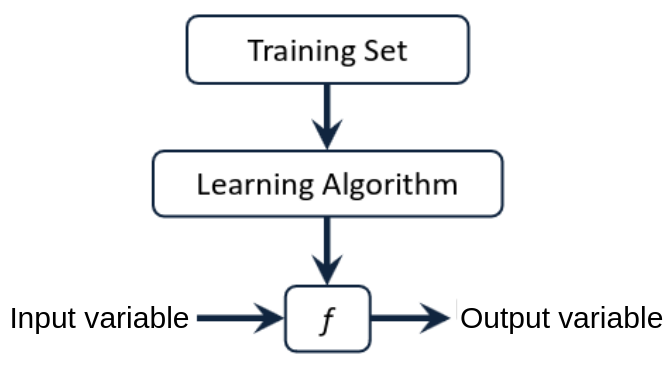
\includegraphics[width=0.5\textwidth]{images/3-model-representation.png}
	\caption{Voorstelling van het model}
	\label{fig:model-representation}
\end{figure}
\noindent
Het model wordt voorgesteld door de volgende vergelijking:
\begin{equation}
	f_{w,b}(x) = w \cdot x + b
	\label{eq:f-wb}
\end{equation}
Hier stelt $x$ de input variabele voor. Parameters $w$ en $b$ stellen het gewicht van de input variabele en de bias-term voor. Deze moeten zo gekozen worden opdat onze voorspelling $f_{w,b}$ de output variabele $y$ zo dicht mogelijk benadert voor onze trainingsdata $(x,y)$. Een ander symbool dat af en toe gebruikt wordt om de predictie voor te stellen is $\hat{y}$. De voorspelling voor één specifiek element uit onze trainingsdata wordt voorgesteld als:
\begin{equation}
	\hat{y}^{(i)}= f_{w,b}(x^{(i)}) = w \cdot x^{(i)} + b
	\label{eq:f-wb-i}
\end{equation}

\subsection{De kostfunctie}
We willen dus dat $\hat{y}$ en $y$ elkaar zo dicht mogelijk benaderen. Om dit te doen stellen we de kostfunctie $J(w,b)$ op:
\begin{equation}
	J(w, b) = \frac{1}{2m}\sum_{}^{m}(f_{w,b}(x^{(i)}) - y^{(i)})^{2}
	\label{eq:cost-function}
\end{equation}
\noindent
Deze kostfunctie (ook wel \textit{squared error function}) is gelijk aan de genormaliseerde totale fout. Om de fout zo klein mogelijk te houden willen we dus de parameters $w$ en $b$ bepalen om de kostfunctie te minimaliseren. Figuur \ref{fig:cost-function} toont onze een visualisatie van de kostfunctie. Zoals we zien op Figuur \ref{fig:cost-function-min}, zal het model de data goed fitten wanneer de kostfunctie minimaal is. De kringen op Figuur \ref{fig:cost-function-not-min} en Figuur \ref{fig:cost-function-min} stellen combinaties van parameters $w$ en $b$ voor die hetzelfde resultaat voor $J(w, b)$ opleveren.

\begin{figure}[h]
	\centering
	\begin{subfigure}{.5\textwidth}
		\centering
		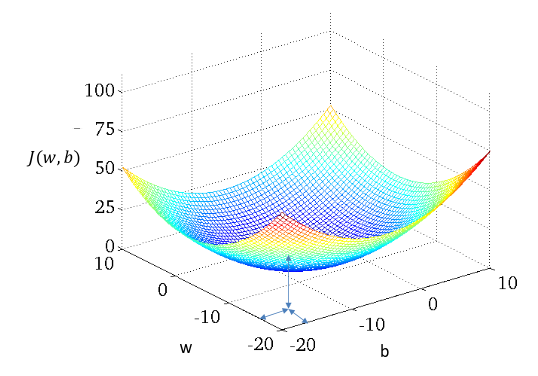
\includegraphics[width=\textwidth]{images/4-cost-function-3d.png}
		\caption{Driedimensionale voorstelling van de kostfunctie}
		\label{fig:cost-function-3d}
	\end{subfigure}
	\begin{subfigure}{.5\textwidth}
		\centering
		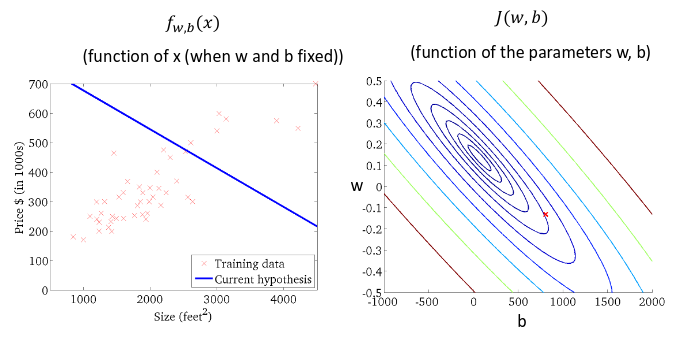
\includegraphics[width=\textwidth]{images/5-cost-function-not-min.png}
		\caption{Niet-geminimaliseerde kostfunctie}
		\label{fig:cost-function-not-min}
	\end{subfigure}
	\begin{subfigure}{.5\textwidth}
		\centering
		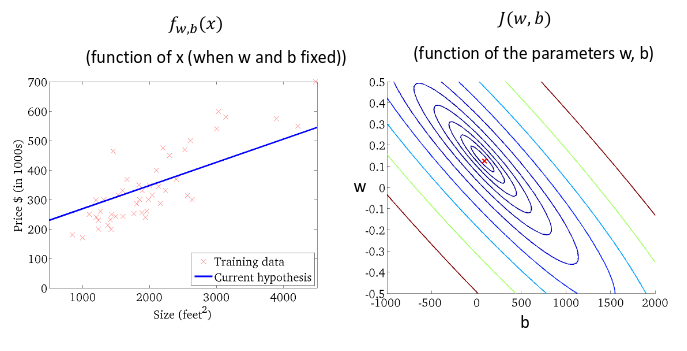
\includegraphics[width=\textwidth]{images/6-cost-function-min.png}
		\caption{Geminimaliseerde kostfunctie}
		\label{fig:cost-function-min}
	\end{subfigure}
	\caption{Grafische voorstelling van de kostfunctie}
	\label{fig:cost-function}
\end{figure}
\newpage
\paragraph{De kostfunctie in Python}
In Python kunnen we de kostfunctie als volgt berekenen:

\begin{lstlisting}
	def compute_cost(x, y, w, b): 
	    """
	    Computes the cost function for linear regression.
	
	    Args:
	        x (ndarray): Shape (m,) Input to the model (City population) 
	        y (ndarray): Shape (m,) Label (Actual profits for the cities)
	        w, b (scalar): Parameters of the model
	        
	    Returns
	        total_cost (float): The cost of using w,b as the parameters for linear regression to fit the data points in x and y
	    """
\end{lstlisting}
\begin{lstlisting}
	    # number of training examples
	    m = x.shape[0] 
	
	    # You need to return this variable correctly
	    total_cost = 0
	
	    # Variable to keep track of sum of cost from each example
	    cost_sum = 0
	
	    # Loop over training examples
	    for i in range(m):
	        # The prediction f_wb for the ith example
	        f_wb = w * x[i] + b
	        # The cost associated with the ith example
	        cost = (f_wb - y[i])**2
	        # Add to sum of cost for each example
	        cost_sum = cost_sum + cost 
	        
	    # Get the total cost as the sum divided by (2*m)
	    total_cost = (1 / (2 * m)) * cost_sum
	
	    return total_cost
\end{lstlisting}

\subsection{\textit{Gradient descent}}

\textit{Gradient descent} is een manier om de kostfunctie te minimaliseren. Hierbij starten we vanaf een bepaalde waarde voor $w$ en $b$ en blijven we deze veranderen om $J(w, b)$ te doen afnemen om zo op een minimum uit te komen. Dit doen we met de gradiënt ($\nabla J = (\frac{\partial J}{\partial w}, \frac{\partial J}{\partial b})$). Deze geeft in de wiskunde de richting van de steilste helling weer. Wiskundig gezien ziet het \textit{gradient descent} algoritme er als volgt uit:

\begin{equation}
	w_{temp} = w - \alpha \frac{\partial}{\partial w} J(w, b)
	\label{eq:w-temp}
\end{equation}
\begin{equation}
	b_{temp} = b - \alpha \frac{\partial}{\partial b} J(w, b)
	\label{eq:b-temp}
\end{equation}
\begin{equation}
	w = w_{temp} 
\end{equation}
\begin{equation}
	b = b_{temp}
\end{equation}
\noindent
We werken met een tijdelijke $w$ en $b$ ($w_{temp}$ en $b_{temp}$) omdat we in onze berekening voor de nieuwe $w$ en $b$ ook gebruik maken van de huidige $w$ en $b$, en we de waarden simultaan willen aanpassen. Indien we geen gebruik zouden maken van deze tijdelijke variabelen, zouden we de geüpdatete versie van $w$ al gebruiken in de berekening van de nieuwe $b$ en dit willen we niet. We zullen de waarden van $w$ en $b$ blijven aanpassen tot we convergentie bereiken. Dit zal betekenen dat we een minimum bereikt hebben. \\
\newline
In formule \ref{eq:w-temp} en formule \ref{eq:b-temp} maken we ook gebruik van de \textit{learning rate} $\alpha$. Dit is een hyperparameter die we goed moeten instellen. Een hyperparameter is niet een parameter die het model definieert, maar wel een parameter die ingesteld moet worden om tot een model te komen. Wanneer $\alpha$ te klein is, zal de \textit{gradient descent} heel langzaam verlopen. Wanneer $\alpha$ te groot is, kan het zijn dat we onze \textit{gradient descent} in te grote stappen uitvoeren en voorbij het minimum schieten. Hierdoor zou het kunnen dat onze convergentie faalt. Het instellen van deze parameter gebeurt typisch in stappen van bijvoorbeeld een factor 3 (0,001 $\rightarrow$ 0,003 $\rightarrow$ 0,01 $\rightarrow$ 0,03 $\rightarrow$ ...). \\
\newline
Een valkuil van dit algoritme is dat we in een lokaal minimum terechtgekomen. Alhoewel dit zelden voorkomt in de praktijk omdat onze modellen in het merendeel van de gevallen convex zijn, gaan we toch even bespreken hoe we dit kunnen verhinderen. Een idee hiervoor is dat we onze initiële gok voor $w$ en $b$ een tiental keer op een willekeurige positie kunnen wagen en dan naar convergentie kunnen gaan. \\
\newline
Wanneer we het minimum van deze random initialisaties nemen, zijn we vrij zeker dat dit het absolute minimum is. Dit is geen waterdicht systeem, maar aangezien de kans op een lokaal minimum klein is, is deze methode voldoende.

\subsection{\textit{Gradient descent} voor lineaire regressie}

Om \textit{gradient descent} toe te passen op lineaire regressie, combineren we formules \ref{eq:f-wb-i}, \ref{eq:cost-function}, \ref{eq:w-temp} en \ref{eq:b-temp}. We bekomen dan de volgende formules:
\begin{equation}
	\frac{\partial}{\partial w}J(w, b) = \frac{1}{m}\sum_{i=1}^{m}(f_{w,b}(x^{(i)}) - y^{(i)}) \cdot x^{(i)}
\end{equation}
\begin{equation}
	\frac{\partial}{\partial b}J(w, b) = \frac{1}{m}\sum_{i=1}^{m}(f_{w,b}(x^{(i)}) - y^{(i)})
\end{equation}
\begin{equation}
	w_{temp} = w - \alpha \frac{1}{m}\sum_{i=1}^{m}(f_{w,b}(x^{(i)}) - y^{(i)}) \cdot x^{(i)}
\end{equation}
\begin{equation}
	b_{temp} = b - \alpha \frac{1}{m}\sum_{i=1}^{m}(f_{w,b}(x^{(i)}) - y^{(i)})
\end{equation}
\noindent
Figuur \ref{fig:gradient-descent} toont ons het resultaat van het uitvoeren van het \textit{gradient descent} algoritme bij een lineaire regressie.
\begin{figure}[h]
	\centering
	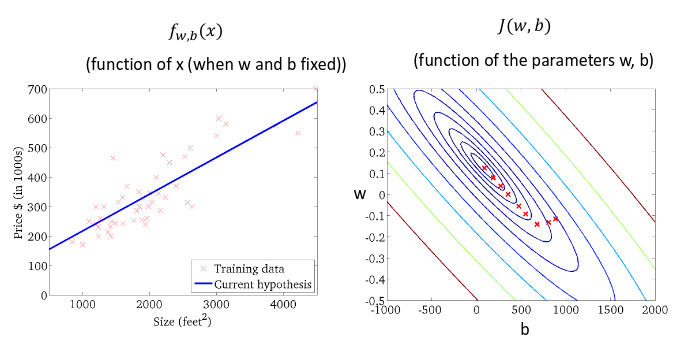
\includegraphics[width=0.6\textwidth]{images/7-gradient-descent.png}
	\caption{\textit{Gradient descent} bij lineaire regressie}
	\label{fig:gradient-descent}
\end{figure}

\paragraph{\textit{Gradient descent} in Python}
In Python kunnen we de gradiënt als volgt berekenen:
\begin{lstlisting}
	def compute_gradient(x, y, w, b): 
	    """
	    Computes the gradient for linear regression 
	    Args:
	        x (ndarray): Shape (m,) Input to the model (City population) 
	        y (ndarray): Shape (m,) Label (Actual profits for the cities)
	        w, b (scalar): Parameters of the model  
	    Returns
	        dj_dw (scalar): The gradient of the cost w.r.t. the parameters w
	        dj_db (scalar): The gradient of the cost w.r.t. the parameter b     
	    """
\end{lstlisting}
\newpage
\begin{lstlisting}
	    # Number of training examples
	    m = x.shape[0]
	
	    # You need to return the following variables correctly
	    dj_dw = 0
	    dj_db = 0
	
	    # Loop over examples
	    for i in range(m):  
	        # The prediction f_wb for the ith example
	        f_wb = w * x[i] + b
	
	        # The gradient for w from the ith example 
	        dj_dw_i = (f_wb - y[i]) * x[i]
	
	        # The gradient for b from the ith example 
	        dj_db_i = f_wb - y[i]
	
	        # Update dj_db
	        dj_db += dj_db_i
	
	        # Update dj_dw
	        dj_dw += dj_dw_i
	
	    # Divide both dj_dw and dj_db by m
	    dj_dw = dj_dw / m
	    dj_db = dj_db / m
	
	    return dj_dw, dj_db
\end{lstlisting}
\noindent
\\
Vervolgens kunnen we deze definitie gebruiken om \textit{gradient descent} uit te voeren:

\begin{lstlisting}
	def gradient_descent(x, y, w_in, b_in, alpha, num_iters): 
	    """
	    Performs batch gradient descent to learn theta. Updates theta by taking num_iters gradient steps with learning rate alpha
	
	    Args:
	        x :    (ndarray): Shape (m,)
	        y :    (ndarray): Shape (m,)
	        w_in, b_in : (scalar) Initial values of parameters of the model
	        alpha : (float) Learning rate
	        num_iters : (int) number of iterations to run gradient descent
	    Returns
	        w : (ndarray): Shape (1,) Updated values of parameters of the model after running gradient descent
	        b : (scalar) Updated value of parameter of the model after running gradient descent
	    """
	
	    # Number of training examples
	    m = len(x)
	
	    # Set initial value to w and b
	    w = copy.deepcopy(w_in)
	    b = b_in
\end{lstlisting}
\newpage
\begin{lstlisting}	
	    for i in range(num_iters):
	        # Calculate the gradient and update the parameters
	        dj_dw, dj_db = compute_gradient(x, y, w, b )  
	
	        # Update Parameters using w, b, alpha and gradient
	        w = w - alpha * dj_dw               
	        b = b - alpha * dj_db               
	
	    return w, b
\end{lstlisting}

\subsection{\textit{Batch gradient descent}}

\textit{Batch gradient descent} is een variant van \textit{gradient descent} waarbij we onze volledige trainingsdata gebruiken in elke stap van het algoritme. Bij \textit{mini-batch} gebruiken we een kleinere deelverzameling van de trainingsdata om een update uit te voeren. 
